\thispagestyle{fancy}
\fancyhead[R]{A.U 2025-2026}
\fancyhead[L]{Chapitre 6 : Sprint 4 -- Orchestration et déploiement continu}

\chapter{Sprint 4 : Orchestration et déploiement continu}

% boîte utilisée pour encadrer les extraits de code (verbatim)
\newsavebox{\manifbox}

\section*{Introduction}
Le Sprint 3 s'est achevé sur une chaîne d'intégration continue capable de produire
automatiquement des images validées et publiées sur un registre. Il reste néanmoins une
étape manuelle : le déploiement effectif de ces images sur le serveur de production.

Le \textbf{Sprint 4}, dernier sprint du projet, referme cette boucle. Il couvre
l'orchestration des conteneurs sur un cluster Kubernetes k3s, la mise en place d'un
déploiement continu selon l'approche GitOps avec Argo CD, la sécurisation des secrets
applicatifs avec HashiCorp Vault, le cloisonnement des droits par RBAC, et enfin la
supervision de l'infrastructure elle-même avec Prometheus et Grafana.

À l'issue de ce sprint, la chaîne DevSecOps est complète : du \textit{commit} du
développeur jusqu'à l'exécution en production, sans aucune intervention manuelle.

\section{Backlog du Sprint 4}
Les \textit{User Stories} retenues pour ce sprint ont été décomposées en tâches
techniques présentées dans le tableau~\ref{tab:backlog-sprint4}.

\renewcommand{\arraystretch}{1.4}
\begin{longtable}{|>{\raggedright\arraybackslash}p{4.1cm}
                  |>{\raggedright\arraybackslash}p{7.7cm}
                  |>{\centering\arraybackslash}p{2.4cm}|}
\hline
\textbf{User Story} & \textbf{Tâches} & \textbf{Estimation} \\
\hline
\endfirsthead

\hline
\textbf{User Story} & \textbf{Tâches} & \textbf{Estimation} \\
\hline
\endhead

\hline
\multicolumn{3}{r}{\textit{Suite du tableau à la page suivante}} \\
\endfoot

\hline
\caption{Backlog du Sprint 4}
\label{tab:backlog-sprint4}
\endlastfoot

En tant que responsable DevSecOps, je veux disposer d'un cluster Kubernetes.
& Installer la distribution k3s sur le VPS OVH. & 2 \\
& Créer l'espace de noms \texttt{monitoring}. & 1 \\
& Configurer l'accès au cluster (\texttt{kubeconfig}). & 1 \\
& Vérifier l'état des n\oe uds et des composants système. & 1 \\
\hline

En tant que responsable DevSecOps, je veux déployer l'application sur le cluster.
& Rédiger les manifestes de déploiement du backend et du frontend. & 2 \\
& Rédiger les manifestes de services de type \texttt{NodePort}. & 1 \\
& Configurer les volumes persistants pour les sauvegardes. & 2 \\
& Injecter la configuration par \texttt{Secret} Kubernetes. & 1 \\
& Vérifier l'accessibilité de l'application depuis l'extérieur. & 1 \\
& Tester le déploiement. & 1 \\
\hline

En tant que responsable DevSecOps, je veux garantir la disponibilité du service.
& Configurer les sondes de vivacité et de disponibilité. & 2 \\
& Définir les demandes et limites de ressources des conteneurs. & 1 \\
& Configurer la stratégie de mise à jour progressive. & 1 \\
& Tester le redémarrage automatique après incident. & 1 \\
\hline

En tant que responsable DevSecOps, je veux automatiser le déploiement (GitOps).
& Installer Argo CD sur le cluster. & 2 \\
& Créer le dépôt Git des manifestes de déploiement. & 1 \\
& Déclarer l'application Argo CD et sa source. & 1 \\
& Activer la synchronisation automatique et l'auto-réparation. & 2 \\
& Développer l'étape Jenkins de mise à jour de l'étiquette d'image. & 2 \\
& Tester le déploiement de bout en bout. & 1 \\
\hline

En tant que responsable DevSecOps, je veux sécuriser les secrets applicatifs.
& Déployer HashiCorp Vault sur le cluster. & 2 \\
& Initialiser et desceller le coffre. & 1 \\
& Migrer les secrets depuis les fichiers de configuration. & 2 \\
& Configurer l'injection des secrets dans les pods. & 2 \\
& Retirer les valeurs sensibles du dépôt Git. & 1 \\
& Tester la récupération des secrets. & 1 \\
\hline

En tant que responsable DevSecOps, je veux cloisonner les droits d'accès.
& Créer les comptes de service applicatifs. & 1 \\
& Définir les rôles et leurs permissions. & 2 \\
& Créer les liaisons entre rôles et comptes de service. & 1 \\
& Appliquer le principe du moindre privilège. & 2 \\
& Tester les restrictions d'accès. & 1 \\
\hline

En tant que responsable DevSecOps, je veux superviser l'infrastructure.
& Déployer Prometheus sur le cluster. & 2 \\
& Configurer la collecte des métriques du cluster. & 2 \\
& Déployer Grafana et le connecter à Prometheus. & 1 \\
& Construire les tableaux de bord de supervision. & 2 \\
& Configurer les règles d'alerte d'infrastructure. & 2 \\
& Tester la remontée des métriques. & 1 \\
\hline

\end{longtable}

\section{Diagramme de cas d'utilisation du Sprint 4}
La figure~\ref{fig:uc-sprint4} présente le diagramme de cas d'utilisation correspondant
aux fonctionnalités développées lors du quatrième sprint.

\begin{figure}[H]
\centering
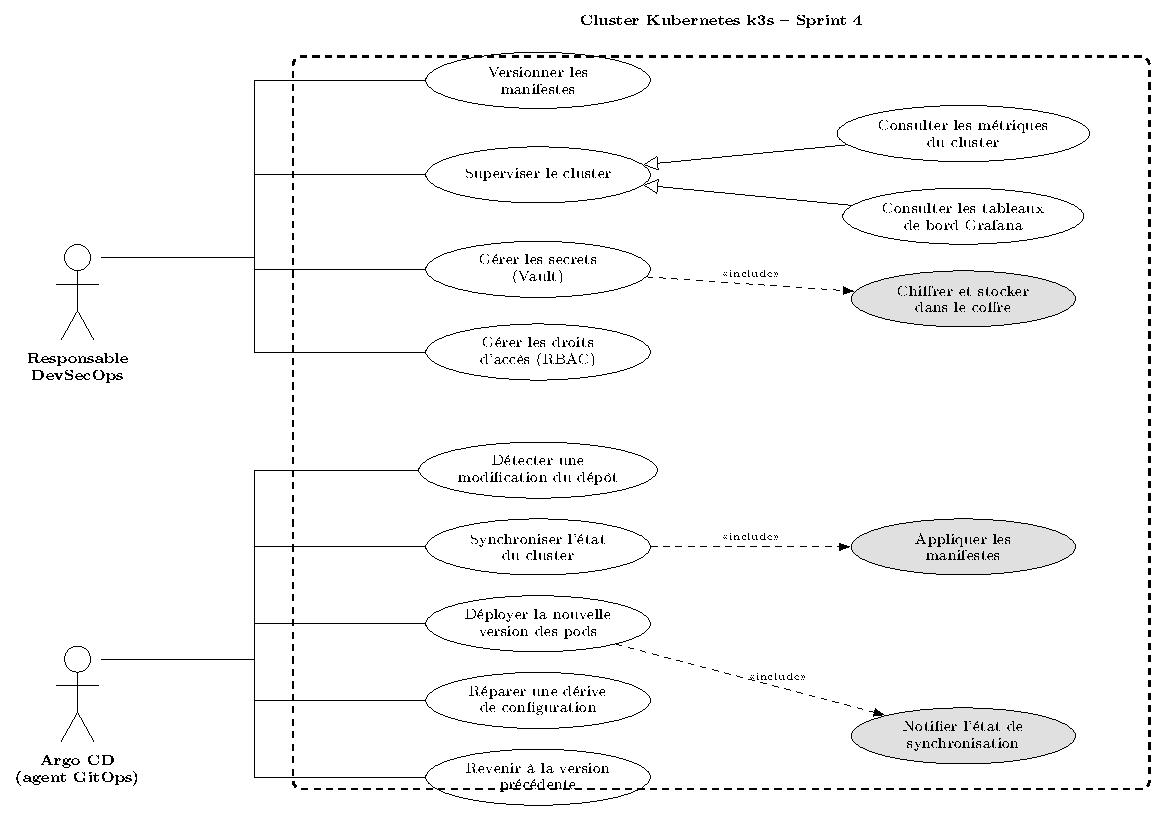
\includegraphics[width=0.96\textwidth]{figures/uc-sprint4.pdf}
\caption{Diagramme de cas d'utilisation du Sprint 4}
\label{fig:uc-sprint4}
\end{figure}

\section{Orchestration avec Kubernetes k3s}
Docker permet d'exécuter un conteneur, mais ne répond pas seul aux besoins d'un
environnement de production : que se passe-t-il si un conteneur s'arrête ? Comment
mettre à jour l'application sans interruption de service ? Comment répartir la charge ?
Kubernetes apporte une réponse à ces questions en orchestrant le cycle de vie des
conteneurs.

La distribution \textbf{k3s} a été retenue plutôt que Kubernetes dans sa version
complète. Il s'agit d'une distribution certifiée conforme, allégée et empaquetée en un
binaire unique d'environ 60 Mo, conçue pour les environnements à ressources limitées.
Elle offre l'intégralité de l'interface de programmation de Kubernetes tout en restant
compatible avec les ressources d'un VPS mutualisé, ce qui correspond exactement au
contexte du projet.

\subsection{Organisation des ressources déployées}
L'ensemble des ressources est regroupé dans un espace de noms dédié nommé
\texttt{monitoring}, qui assure un cloisonnement logique vis-à-vis des composants
système du cluster. Le tableau~\ref{tab:k8s-res} récapitule les ressources déployées.

\renewcommand{\arraystretch}{1.3}
\small
\begin{longtable}{|>{\raggedright\arraybackslash}p{3.4cm}
                  |>{\raggedright\arraybackslash}p{3.0cm}
                  |>{\raggedright\arraybackslash}p{7.0cm}|}
\hline
\textbf{Ressource} & \textbf{Type} & \textbf{Rôle} \\
\hline
\endfirsthead

\hline
\textbf{Ressource} & \textbf{Type} & \textbf{Rôle} \\
\hline
\endhead

\hline
\caption{Ressources Kubernetes déployées dans l'espace de noms \texttt{monitoring}}
\label{tab:k8s-res}
\endlastfoot

\texttt{frontend} & \texttt{Deployment} & Exécuter et maintenir le pod du frontend React servi par Nginx. \\
\hline
\texttt{frontend} & \texttt{Service} & Exposer le frontend à l'extérieur du cluster sur le port 30080. \\
\hline
\texttt{backend} & \texttt{Deployment} & Exécuter et maintenir le pod du backend Node.js. \\
\hline
\texttt{backend} & \texttt{Service} & Exposer l'API REST et le canal WebSocket sur le port 30300. \\
\hline
\texttt{monitoring-secret} & \texttt{Secret} & Injecter la configuration sensible dans le pod du backend. \\
\hline
\texttt{backups-pvc} & \texttt{Persistent}\allowbreak\texttt{VolumeClaim} & Conserver les archives de sauvegarde indépendamment du cycle de vie des pods. \\
\hline
\texttt{argocd} & \textit{espace de noms} & Héberger les composants du contrôleur de déploiement continu. \\
\hline
\texttt{vault} & \textit{espace de noms} & Héberger le coffre-fort de secrets. \\
\hline
\texttt{monitoring-sys} & \textit{espace de noms} & Héberger Prometheus et Grafana. \\
\hline

\end{longtable}
\normalsize

\subsection{Manifeste de déploiement du backend}
La figure~\ref{fig:manifest-back} présente le manifeste de déploiement du backend. Le
champ \texttt{image} référence l'image publiée par le \textit{pipeline} du Sprint 3,
étiquetée par le numéro de build ; c'est précisément cette étiquette que le
\textit{pipeline} met à jour pour déclencher un nouveau déploiement.

\begin{lrbox}{\manifbox}
\begin{minipage}{0.88\textwidth}
\begin{verbatim}
apiVersion: apps/v1
kind: Deployment
metadata:
  name: backend
  namespace: monitoring
spec:
  replicas: 1
  selector:
    matchLabels:
      app: backend
  template:
    metadata:
      labels:
        app: backend
    spec:
      containers:
      - name: backend
        image: mariemchaabani/monitoring-backend:39
        ports:
        - containerPort: 3000
        envFrom:
        - secretRef:
            name: monitoring-secret
        volumeMounts:
        - name: backups
          mountPath: /app/backups
      volumes:
      - name: backups
        persistentVolumeClaim:
          claimName: backups-pvc
\end{verbatim}
\end{minipage}
\end{lrbox}
\begin{figure}[H]
\centering
\fbox{\usebox{\manifbox}}
\caption{Manifeste de déploiement du backend}
\label{fig:manifest-back}
\end{figure}

\subsection{Exposition des services}
Les deux applications sont exposées par des services de type \texttt{NodePort}, qui
ouvrent un port fixe sur l'adresse du n\oe ud. Cette solution a été retenue pour sa
simplicité de mise en \oe uvre sur un cluster mono-n\oe ud, où le recours à un
équilibreur de charge externe ne se justifierait pas.

\begin{lrbox}{\manifbox}
\begin{minipage}{0.88\textwidth}
\begin{verbatim}
apiVersion: v1
kind: Service
metadata:
  name: backend
  namespace: monitoring
spec:
  selector:
    app: backend
  ports:
  - port: 3000
    targetPort: 3000
    nodePort: 30300
  type: NodePort
\end{verbatim}
\end{minipage}
\end{lrbox}
\begin{figure}[H]
\centering
\fbox{\usebox{\manifbox}}
\caption{Manifeste du service d'exposition du backend}
\label{fig:manifest-svc}
\end{figure}

L'application est ainsi accessible à l'adresse \texttt{http://}\allowbreak\texttt{141.227.129.194:30080}
pour l'interface web et \texttt{http://}\allowbreak\texttt{141.227.129.194:30300} pour l'API, cette dernière
étant également l'adresse consommée par l'application mobile.

\section{Déploiement continu avec Argo CD}
Le \textit{pipeline} du Sprint 3 s'arrête à la publication de l'image. L'approche
\textbf{GitOps} complète cette chaîne en posant un principe simple : \emph{le dépôt Git
constitue l'unique source de vérité de l'état souhaité du cluster}. Toute modification de
l'infrastructure passe obligatoirement par un \textit{commit}, ce qui la rend versionnée,
revue et réversible.

Argo CD est le contrôleur qui met ce principe en application. Déployé dans le cluster, il
compare en permanence l'état réel du cluster à l'état décrit dans le dépôt Git et corrige
automatiquement tout écart.

\subsection{Fonctionnement de la chaîne complète}
La figure~\ref{fig:gitops} illustre l'enchaînement complet, du \textit{commit} du
développeur jusqu'à l'exécution en production.

\begin{figure}[H]
\centering
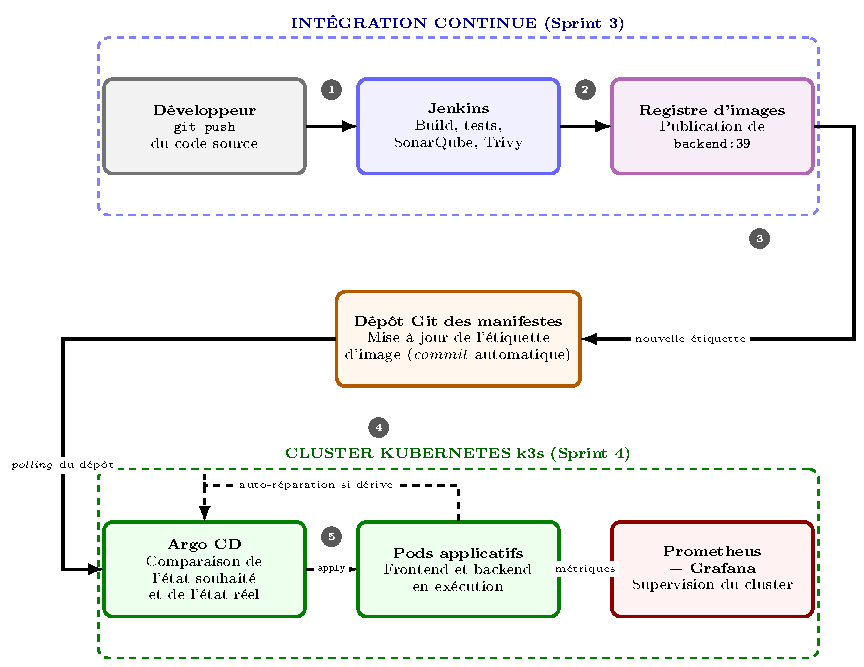
\includegraphics[width=\textwidth]{figures/gitops.pdf}
\caption{Chaîne de déploiement continu selon l'approche GitOps}
\label{fig:gitops}
\end{figure}

Concrètement, la séquence est la suivante : le développeur pousse son code ; Jenkins le
construit, le valide et publie une image étiquetée par le numéro de build ; le
\textit{pipeline} met alors à jour cette étiquette dans le dépôt de manifestes ; Argo CD
détecte ce nouveau \textit{commit}, constate l'écart entre l'état souhaité et l'état réel
du cluster, et applique les manifestes ; Kubernetes procède enfin à une mise à jour
progressive des pods.

\subsection{Auto-réparation et retour arrière}
Deux options ont été activées sur l'application Argo CD :

\begin{itemize}[label=\ding{43}]
  \item la \textbf{synchronisation automatique}, qui applique les manifestes dès la
        détection d'un nouveau \textit{commit}, sans validation manuelle ;
  \item l'\textbf{auto-réparation}, qui annule toute modification appliquée directement
        sur le cluster sans passer par le dépôt Git. Une intervention manuelle en
        production est ainsi automatiquement reprise, ce qui garantit que le dépôt reste
        le reflet fidèle de l'état réel.
\end{itemize}

Le retour arrière découle naturellement de ce fonctionnement : revenir à une version
antérieure ne requiert aucune procédure particulière, il suffit d'annuler le
\textit{commit} correspondant dans le dépôt de manifestes.

\section{Gestion des secrets avec HashiCorp Vault}
La configuration de l'application comporte plusieurs valeurs sensibles : chaîne de
connexion à MongoDB Atlas, identifiants du serveur SMTP, clé de signature des jetons JWT
et identifiants du compte administrateur.

Dans un déploiement Kubernetes classique, ces valeurs sont placées dans une ressource
\texttt{Secret}. Or ce mécanisme n'offre qu'un encodage en base 64, aisément réversible :
un tel manifeste versionné dans un dépôt Git expose donc les identifiants en clair à
toute personne y ayant accès, et ce de manière définitive dans l'historique.

\textbf{HashiCorp Vault} répond à cette limite en centralisant les secrets dans un coffre
chiffré. Les manifestes versionnés ne contiennent plus que des \emph{références} vers le
coffre, tandis que les valeurs réelles sont injectées dans le pod au moment de son
démarrage. Le tableau~\ref{tab:vault} présente les secrets ainsi externalisés.

\renewcommand{\arraystretch}{1.3}
\begin{longtable}{|>{\raggedright\arraybackslash}p{4.6cm}
                  |>{\raggedright\arraybackslash}p{9.2cm}|}
\hline
\textbf{Secret} & \textbf{Usage} \\
\hline
\endfirsthead

\hline
\textbf{Secret} & \textbf{Usage} \\
\hline
\endhead

\hline
\caption{Secrets applicatifs externalisés dans Vault}
\label{tab:vault}
\endlastfoot

\texttt{MONGODB\_URI} & Chaîne de connexion authentifiée à la base MongoDB Atlas. \\
\hline
\texttt{JWT\_SECRET} & Clé de signature et de vérification des jetons d'authentification. \\
\hline
\texttt{EMAIL\_USER} / \texttt{EMAIL\_PASS} & Identifiants du compte SMTP d'envoi des notifications. \\
\hline
\texttt{ADMIN\_EMAIL} / \texttt{ADMIN\_PASSWORD} & Identifiants du compte administrateur initial. \\
\hline
\texttt{SSH\_PASSWORD} & Mot de passe utilisé pour les actions à distance sur les serveurs supervisés. \\
\hline

\end{longtable}

Cette externalisation apporte trois bénéfices : le dépôt Git ne contient plus aucune
valeur sensible, la rotation d'un secret ne nécessite plus de reconstruire une image, et
chaque accès au coffre est journalisé, ce qui satisfait aux exigences d'auditabilité.

\section{Contrôle d'accès avec RBAC}
Par défaut, un pod dispose de droits plus étendus que nécessaire sur l'interface de
programmation du cluster. Le mécanisme \textbf{RBAC} (\textit{Role-Based Access Control})
permet d'appliquer le principe du \textbf{moindre privilège} : chaque composant ne reçoit
que les permissions strictement indispensables à son fonctionnement.

Trois niveaux de droits ont été définis, présentés dans le tableau~\ref{tab:rbac}.

\renewcommand{\arraystretch}{1.3}
\begin{longtable}{|>{\raggedright\arraybackslash}p{3.8cm}
                  |>{\raggedright\arraybackslash}p{4.4cm}
                  |>{\raggedright\arraybackslash}p{5.6cm}|}
\hline
\textbf{Compte de service} & \textbf{Portée} & \textbf{Permissions accordées} \\
\hline
\endfirsthead

\hline
\textbf{Compte de service} & \textbf{Portée} & \textbf{Permissions accordées} \\
\hline
\endhead

\hline
\caption{Rôles RBAC définis sur le cluster}
\label{tab:rbac}
\endlastfoot

\texttt{backend-sa} & Espace de noms \texttt{monitoring} & Lecture seule des \texttt{Secret} et \texttt{ConfigMap} de son espace de noms. \\
\hline
\texttt{argocd-controller} & Cluster entier & Création, modification et suppression des ressources applicatives. \\
\hline
\texttt{prometheus-sa} & Cluster entier & Lecture seule des pods, services et n\oe uds pour la collecte des métriques. \\
\hline

\end{longtable}

Le compte de service du backend illustre bien cette démarche : il peut lire les secrets
dont il a besoin, mais ne peut ni les modifier, ni consulter les ressources des autres
espaces de noms, ni agir sur les pods du cluster. En cas de compromission du conteneur,
la portée de l'attaque reste ainsi strictement circonscrite.

\section{Supervision de l'infrastructure avec Prometheus et Grafana}
La plateforme développée supervise les \emph{serveurs}. Il restait à superviser
l'\emph{infrastructure} qui l'héberge, c'est-à-dire le cluster lui-même. Cette
supervision de second niveau est assurée par le couple Prometheus et Grafana.

Prometheus collecte périodiquement les métriques exposées par les composants du cluster
et les conserve dans une base de séries temporelles. Grafana s'y connecte comme source de
données et restitue ces métriques sous forme de tableaux de bord. Les indicateurs
supervisés sont récapitulés dans le tableau~\ref{tab:prom}.

\renewcommand{\arraystretch}{1.3}
\begin{longtable}{|>{\raggedright\arraybackslash}p{4.4cm}
                  |>{\raggedright\arraybackslash}p{9.4cm}|}
\hline
\textbf{Catégorie} & \textbf{Indicateurs supervisés} \\
\hline
\endfirsthead

\hline
\textbf{Catégorie} & \textbf{Indicateurs supervisés} \\
\hline
\endhead

\hline
\caption{Indicateurs supervisés par Prometheus}
\label{tab:prom}
\endlastfoot

N\oe ud du cluster & Charge processeur, mémoire disponible, espace disque, charge système. \\
\hline
Pods applicatifs & État d'exécution, nombre de redémarrages, consommation processeur et mémoire par conteneur. \\
\hline
Kubernetes & Nombre de pods par état, disponibilité des déploiements, événements du cluster. \\
\hline
Application & Nombre de requêtes traitées, temps de réponse de l'API, nombre de connexions WebSocket actives. \\
\hline

\end{longtable}

Des règles d'alerte ont par ailleurs été définies afin de notifier l'équipe en cas de
redémarrages répétés d'un pod, d'indisponibilité d'un déploiement ou de saturation des
ressources du n\oe ud.

Cette supervision d'infrastructure est complémentaire de la plateforme développée : cette
dernière surveille les serveurs applicatifs du parc, tandis que Prometheus et Grafana
surveillent le socle technique qui l'exécute.

\section{Réalisation du Sprint 4}

\begin{itemize}[label=\ding{220}]
\item \textbf{État du cluster k3s :}
\end{itemize}
La figure~\ref{fig:real-k3s} présente l'état des pods déployés dans l'espace de noms
\texttt{monitoring}, avec leur statut, leur nombre de redémarrages et leur durée
d'exécution.

\begin{figure}[H]
    \centering
    \includegraphics[width=0.95\textwidth]{Image/real-k3s-pods.png}
    \caption{État des pods déployés sur le cluster k3s}
    \label{fig:real-k3s}
\end{figure}

\begin{itemize}[label=\ding{220}]
\item \textbf{Interface Argo CD :}
\end{itemize}
La figure~\ref{fig:real-argo} illustre l'interface d'Argo CD. L'arborescence des
ressources y est représentée graphiquement, accompagnée de l'état de santé de
l'application et de son état de synchronisation avec le dépôt Git.

\begin{figure}[H]
    \centering
    \includegraphics[width=0.95\textwidth]{Image/real-argocd.png}
    \caption{Interface de synchronisation Argo CD}
    \label{fig:real-argo}
\end{figure}

\begin{itemize}[label=\ding{220}]
\item \textbf{Coffre-fort HashiCorp Vault :}
\end{itemize}
La figure~\ref{fig:real-vault} présente l'interface de Vault et l'arborescence des
secrets applicatifs stockés dans le coffre.

\begin{figure}[H]
    \centering
    \includegraphics[width=0.9\textwidth]{Image/real-vault.png}
    \caption{Interface de gestion des secrets HashiCorp Vault}
    \label{fig:real-vault}
\end{figure}

\begin{itemize}[label=\ding{220}]
\item \textbf{Tableau de bord Grafana :}
\end{itemize}
La figure~\ref{fig:real-grafana} illustre le tableau de bord Grafana de supervision du
cluster, alimenté par Prometheus.

\begin{figure}[H]
    \centering
    \includegraphics[width=0.95\textwidth]{Image/real-grafana.png}
    \caption{Tableau de bord Grafana de supervision du cluster}
    \label{fig:real-grafana}
\end{figure}

\begin{itemize}[label=\ding{220}]
\item \textbf{Application déployée en production :}
\end{itemize}
La figure~\ref{fig:real-prod} présente la plateforme accessible en production à l'adresse
\texttt{http://}\allowbreak\texttt{141.227.129.194:30080}, servie par les pods du cluster k3s.

\begin{figure}[H]
    \centering
    \includegraphics[width=0.95\textwidth]{Image/real-production.png}
    \caption{Plateforme déployée en production sur le cluster}
    \label{fig:real-prod}
\end{figure}

\section*{Conclusion}
Ce chapitre a présenté les travaux réalisés lors du Sprint 4, dernier sprint du projet.
Celui-ci a permis d'orchestrer les conteneurs applicatifs sur un cluster Kubernetes k3s,
d'automatiser intégralement le déploiement selon l'approche GitOps avec Argo CD, de
sécuriser les secrets applicatifs dans un coffre HashiCorp Vault, de cloisonner les
droits d'accès par RBAC et de superviser l'infrastructure avec Prometheus et Grafana.

La chaîne DevSecOps est désormais complète : un \textit{commit} poussé par le développeur
déclenche automatiquement la construction, les tests, l'analyse de qualité, l'analyse de
sécurité, la publication de l'image puis son déploiement en production, sans aucune
intervention manuelle et sans interruption de service.
